% keisoku_report.tex  計測制御のレポートの雛型
\documentclass{jarticle}
\usepackage{listings,jlisting}  % ソースコードを行番号付きで載せるパッケージ
\usepackage{color}              % 色付けするパッケージ
\usepackage[dvipdfmx]{graphicx}         % 画像を張り込むパッケージ
\setlength{\topmargin}{0mm}
\setlength{\oddsidemargin}{0mm}
\setlength{\textwidth}{16cm}
\setlength{\textheight}{23cm}

%\renewcommand{\lstlistingname}{リスト} % 「ソースコード」を変更する
\lstset{language=C,% ソースの種類の指定
        basicstyle=\footnotesize,% リスト全体の設定
        commentstyle=\color{blue}\textit,% コメント部分の設定
        keywordstyle=\textbf,%  C言語の予約語(if,for,while等)の設定
        %keywordstyle=\color{red}\bfseries,%
        classoffset=1,%
        breakindent=20pt,%    改行時インデント量。デフォルト:20pt。
        breaklines=true,%   行が長くなってしまった場合の改行。
        frame=tlRB,framesep=7pt,% frame は top,left,right,bottom の1文字で指定、大文字は二重線
        showstringspaces=false,% string 中のスペースを記号表示するか
        numbers=left,% 行番号を付ける位置
        %stepnumber=2,%  何行ごとに行番号を表示するか デフォルトは 1
        numberstyle=\scriptsize\color{blue}% 行番号の表示スタイル
        }%

\begin{document}

\section{実験の目的}

現在ではほとんどの通信機器が計算機から制御できるようになっている。
世界で誰も行なっていない計測を行うためには、自分でソフトウェア開発を
することが必要となる。
本実験の目的は、プログラミング言語としては C言語を用い、
計算機から外部機器を制御する基本的な考え方とその方法を学ぶことである。

\section{実験の方法}
C言語を用いて、課題1〜11に取り組んだ。

\section{実験}

%次のように、\lstinputlisting で外部ファイルを指定することもできる。
% この場合は、元のソースが変更されても、自動的に変更される。

\subsection{実験1}
10進数を2進数に変換するプログラムを作成した。10進数を2で割った余りを
配列に代入して、商がゼロになるまで繰り返した。

\lstinputlisting[caption=10進数を2進数へ変換,label=list:on-led]{c_pro/decbin.c}

\subsection{実験2}
\subsubsection{方法}
CPU処理時間の測定を行なった。入力した回数だけforループを回すように設計した。関数の引数とforループの変数の型をlong型からlonglong型にした場合の処理時間の差異も検証した。clock-gettime関数を使用するため、time.hをincludeし、コンパイル時に-lrtとリンクをした。

\lstinputlisting[caption=CPU処理時間の計測,label=list:on-led]{c_pro/j2.c}

\subsubsection{結果}

\begin{table}[h]
   \begin{center}

       \caption{forループ回数および変数の型の違いにおける処理時間}
        \begin{tabular}{|r|r|r|}
         \hline
         ループ回数[回] & long型[sec] & long lomg 型[sec]\\
         \hline
         $10^0$ & 0.000003  & 0.000003 \\
         $10^1$ & 0.000003  & 0.000003 \\
         $10^2$ & 0.000003  & 0.000004 \\
         $10^3$ & 0.000005  & 0.000011 \\
         $10^4$ & 0.000023  & 0.000083 \\
         $10^5$ & 0.000203  & 0.000803 \\
         $10^6$ & 0.002026  & 0.008032 \\
         $10^7$ & 0.020057  & 0.083567 \\
         $10^8$ & 0.203523  & 0.835881 \\
         $10^9$ & 2.050905  & 8.041809 \\
         \hline
        \end{tabular}
       \label{table:Cs137}

   \end{center}
  \end{table}
  
  グラフを図\ref{fig:fig2} に示す。図の直線はループ回数$10^4$以降のデータによって得られた回帰直線である。
  
\begin{figure}[ht]
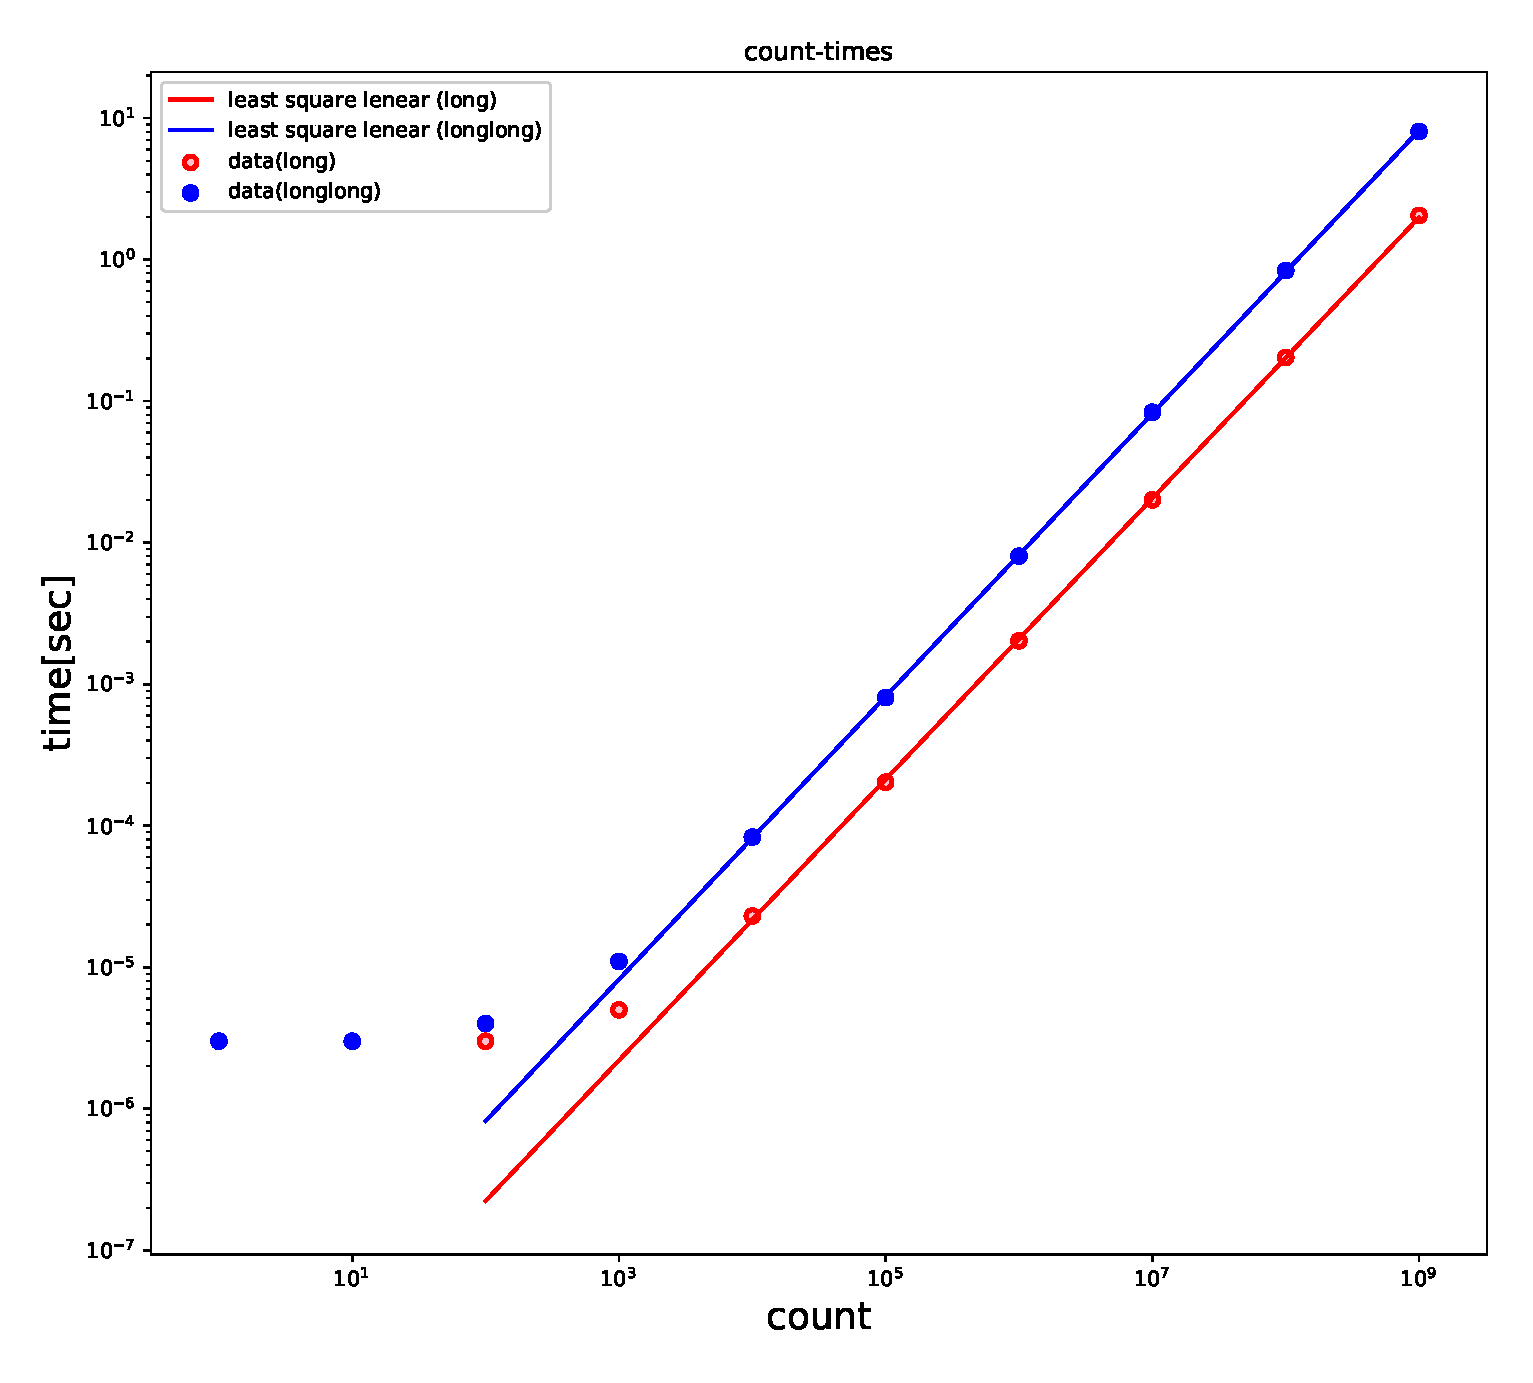
\includegraphics[width=0.8\textwidth]{fig/fig2.eps}
\caption{forループ回数における処理速度}
\label{fig:fig2}
\end{figure}

\subsubsection{考察}
図\ref{fig:fig2}より、処理時間がループ回数に比例していることが読み取れる。$10^3$未満のデータが直線上にのらない要因はfor文以外に,ある一定の処理時間が生じているためだと考えられる。\\
forループ1回あたりの時間は回帰直線よりlong型は$2.05 \times 10^{-9}[sec]$,longlong型は$8.04 \times 10^{-9}[sec]$であると考えられる。
実験で用いたCPUのクロック数は2.00[GHz]であるので1回の処理時間は
$0.5 \times 10^{-9}[sec]$である。ゆえに計測の際の処理時間はこの整数倍であるので、long型は$2.05 \times 10^{-9}[sec]$で4回,longlong型は$8.04 \times 10^{-9}[sec]$で16回の処理が行われていると考えられる。


\subsection{実験3}
実験3〜10ではデジタル入力ボードを用いて実験を行った。これを制御する関数を用いるため、fbippi.hをincludeし、コンパイル時に-lgpg2746とリンクをした。

\lstinputlisting[caption=,label=list:on-led]{c_pro/on_led.c}

\subsection{実験4}

\lstinputlisting[caption=,label=list:on-led]{c_pro/j4.c}

\subsection{実験5}

\lstinputlisting[caption=,label=list:on-led]{c_pro/j5.c}

\subsection{実験6}

\lstinputlisting[caption=,label=list:on-led]{c_pro/j6.c}

\subsection{実験7}

\lstinputlisting[caption=,label=list:on-led]{c_pro/j7.c}

\subsection{実験8}
\subsubsection{方法}

\lstinputlisting[caption=,label=list:on-led]{c_pro/j8.c}

\subsubsection{結果}
\begin{table}[h]
   \begin{center}

       \caption{総点灯回数における各LEDの点灯回数}
        \begin{tabular}{|r|r|r|r|r|}
         \hline
         総点灯回数[回] & 平均回数[回] & 標準偏差[回] & 出現確率 &誤差率\\
         \hline
         $10^2$ & 49.2  & 5.1 & 0.492 & 0.051\\
         $10^3$ & 49.2  & 5.1 & 0.492 & 0.051\\
         $10^4$ & 4984.3  & 49.4 & 0.498 & 0.049\\
         $10^5$ & 50061.5  & 179.5 & 0.500 & 0.018\\
         \hline
        \end{tabular}
       \label{table:Cs137}

   \end{center}
  \end{table}
  
\subsubsection{考察}
総点灯回数が増加するごとに出現確率が0.5に近づき,
誤差率が減少していくことが読み取れる。\\
\\

\subsection{実験9}
\subsubsection{方法}

\lstinputlisting[caption=,label=list:on-led]{c_pro/j9.c}

\subsubsection{結果}

\begin{table}[h]
   \begin{center}

       \caption{ステップモータの回転}
        \begin{tabular}{|r|r|r|r|}
         \hline
         & 360度回転[step] & 1step[deg] & 最小間隔[$\mu s$]\\
         \hline
         $1相励磁$ & 48  & 0.133 & 6300\\
         $2相励磁$ & 48  & 0.133 & 4600\\
         $1-2相励磁$ & 96  & 0.267 & 2400\\         
         \hline
        \end{tabular}
       \label{table:Cs137}

   \end{center}
  \end{table}

\subsubsection{考察}
動作原理より1-2相励磁は、1相励磁に比べ1stepあたりの回転角度が小さいことが分かる。実験によりこのことが確かめられた。

\subsection{実験10}

\lstinputlisting[caption=,label=list:on-led]{c_pro/j10.c}

\subsection{実験11}

\lstinputlisting[caption=,label=list:on-led]{c_pro/j11.c}

12行目のH0をH1に帰ると、ヘッダが現れた。

\section{全体の感想}
例題から取り組み始めたため、課題を全て終了することはできなかったが、C言語および
計算機制御について、深く学ぶことができた。私は普段、スクリプト言語であるPythonを使うことが多い。
そのためセミコロン等のつけ忘れなどによる文法エラー、コンパイル時のミス、型宣言など、基本的な点で
つまづくことが多かったように思う。今回の実験を通してプログラミングの基礎を学び直せたのは非常によかった。
また個人的にC言語と各言語との違いを調べルコとで、C言語がPHPやJavaScriptなどに大きな影響を与えていることも学べた。


\end{document}
